\documentclass[conference]{IEEEtran}
\IEEEoverridecommandlockouts
% The preceding line is only needed to identify funding in the first footnote. If that is unneeded, please comment it out.
\usepackage{cite}
\usepackage{amsmath,amssymb,amsfonts}
\usepackage{cleveref}
\usepackage{algorithmic}
\usepackage{graphicx}
\usepackage{textcomp}
\usepackage{xcolor}
\def\BibTeX{{\rm B\kern-.05em{\sc i\kern-.025em b}\kern-.08em
    T\kern-.1667em\lower.7ex\hbox{E}\kern-.125emX}}
\begin{document}

\title{Towards a system for Adaptive sampling of processes floating with the current*\\
{\footnotesize \textsuperscript{*}Note: Working title}
%\thanks{Identify applicable funding agency here. If none, delete this.}
}

\author{\IEEEauthorblockN{
Andreas Våge\IEEEauthorrefmark{1},
Tor Nordam\IEEEauthorrefmark{2},
Aya Saad\IEEEauthorrefmark{1},
Annette Stahl\IEEEauthorrefmark{1},
Martin Ludvigsen\IEEEauthorrefmark{3},
Kanna Rajan\IEEEauthorrefmark{4},
}
\IEEEauthorblockA{\IEEEauthorrefmark{1}
\textit{Dept. of Engineering Cybernetics},
\textit{Norwegian University of Science and Technology (NTNU)},
Trondheim, Norway \\
}
\IEEEauthorblockA{\IEEEauthorrefmark{2}
\textit{Dept. of Environment and New Resources},
\textit{SINTEF Ocean},
Trondheim, Norway \\
}
\IEEEauthorblockA{\IEEEauthorrefmark{3}
\textit{Dept. of Marine Technology},
\textit{NTNU},
Trondheim, Norway \\
}
\IEEEauthorblockA{\IEEEauthorrefmark{4}
\textit{Underwater Systems and Technology Laboratory},
\textit{ University of Porto},
Porto,  Portugal \\
}
}
\maketitle

\begin{abstract}

\end{abstract}

\begin{IEEEkeywords}
AUV, AI, Planning, Plankton, Gaussian Process
\end{IEEEkeywords}

\section{Introduction}
Planktonic biomass forms the fundamental food source for consumers at higher trophic levels. They play a significant role in producing more than $50\%$ of the global oxygen supply. Hence, studying their community structure, abundance, and dispersion across the ocean is a primary research concern. To avoid transferring planktonic organisms to the lab or applying ship-based point profiling as traditional approaches suggest, we propose, in this paper, a framework that aims at measuring targeted plankton taxa in-situ. 
The framework initially identifies target taxa hotpots related to the upper water-column microbial biology. Then, it adaptively plans the tracking of the suggested hotspots for further exploration, allowing for accurate modeling of targeted biological phenomena, which is an essential task for marine biologists and the management of marine ecology.
%Big picture stuff..

\textbf{AILARON} (\textbf{A}utonomous
\textbf{I}maging and \textbf{L}earning \textbf{A}i \textbf{RO}bot
identifying pla\textbf{N}kton taxa in-situ)

\section{Motivation}
Following processes along the current in the ocean is useful..
I.e. for AILARON it is very useful tool for biologists.. 

\section{Related Work}
Earlier work on robotic adaptive sampling in the upper water column typically models the temporal property caused by the current as noise under the assumption that the sample time-span is short enough compared to the current velocity so that the transportation is negligible or the current and the process being observed are in a stationary equilibrium.
Incorporating the current into the model is ambitious, but numerical ocean models provides more accurate forecasts and small and improved acoustic sensors allows AUVs to directly measure local current profiles.


The following section describes one attempt to estimate and include the current into the models used for adaptive sampling; enabling the AUV to follow interesting processes along the current over time.

\section{Technical Description}
In the AILARON project the process monitored are microbial biology in the upper water column, and a novel silhouette camera has been implemented into the hull of a AUV.
It continuously captures images of particles floating trough its capture volume, magnifying them while keeping them in focus.
The raw images are processed and classified by a state-of-the-art deep learning model on-board the AUV, resulting in a stream of detected particle classes along with prediction confidences.
This stream is accumulated and interpreted as concentration measurements of the different classes with accompanying measurement variances.

For now we only consider one feature at a time, i.e. the total concentration of particles, but extending the system to multiple classes is possible.
Also other observable processes then microbial biology could be monitored with the same system. 

The overall sense, plan and act loop for the AILARON project is seen in \cref{fig:sensePlanActLoop}

\begin{figure}[tbp]
\centerline{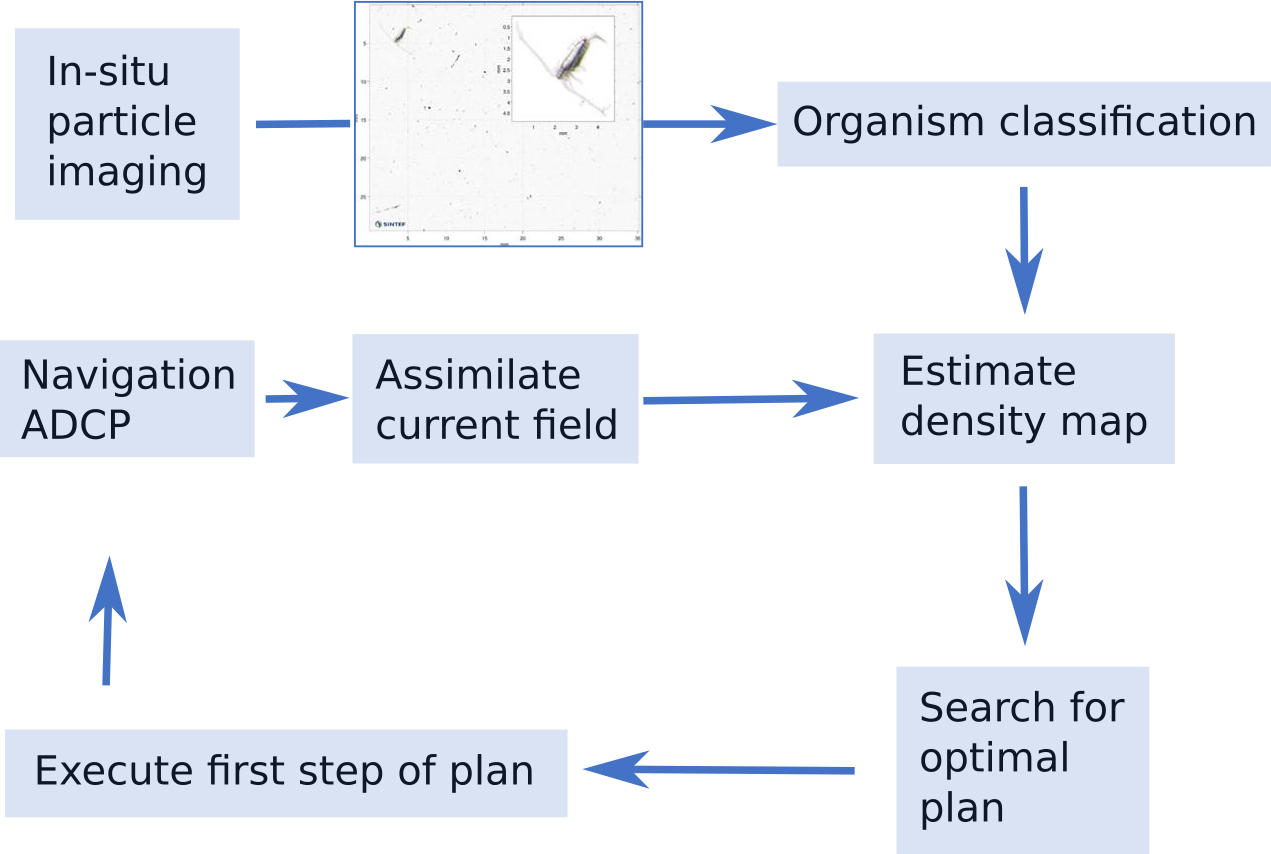
\includegraphics[width=0.9\linewidth]{figures/workflow-simplified.png}}
\caption{The overall control loop running on board the AUV in the AILARON project.}
\label{fig:sensePlanActLoop}
\end{figure}

\paragraph{Local Current Model}
The novel integration of a local current model allows our method to sample a process over a long duration, while taking into account the transport of the process along the current.
The local current model is either estimated prior to the mission from the Numerical hydrodynamic model SINMOD or accumulated during the mission from acoustic doppler current profiler (ADCP) measurements on the AUV.

\paragraph{Particle Transportation}
An ensemble of particles are drawn from the estimated sample area. 
Each particle is transported individually, using a variable-time step integrator through the current field, applying a random walk with the local diffusivity.

\paragraph{Gaussian Process}
Kriging/Gaussian Process regression is performed over the transported particles.
Gaussian process regression is data driven and requires very few parameters, which is important as the process observed is little known, making it hard to fit a parameter based model.
In addition to estimate the mean predicted values (the Kriging surface) Gaussian Process regression also estimates the uncertainty, which is later used to balance exploration vs exploitation when deliberating where the AUV should go next.

\paragraph{Objective Function}
The objective function is calculated over the estimated GP model along the path candidate.
It is based on three interests:
\begin{itemize}
    \item scientific interest in particular plankton classes.
    \item Exploitation: maximise expected measured concentration according to the kriging surface.
    \item Exploration: minimise model variance by sampling from previously little visited areas.
\end{itemize}

\paragraph{Path Heuristics}
The goal is to find the path which maximises the objective function based on the estimated GP model.
Only the first part of the path will be traversed before new measurements are incorporated into the model and a new path is deliberated, however the path should be longer than the first step to achieve long term goals.
However allowing any kind of path requires infinite evaluations of the objective function.
The search is made more efficient by utilising traditional survey paths as heuristics. E.g the standard square survey showed in Fig.~\ref{fig:munkholmen} is parameterised by the covered rectangle and its density, which is significantly fewer parameters to optimise compared to specifying each line individually. 
%Bresenham's line algorithm

All code is open source and based on open source projects. Including the AUV control and navigation software (DUNE) and mission control (Neptus). 

\section{Experimental Results}
The system has been tested and verified in simulations and on historic data. Fig.~\ref{fig:munkholmen} shows the planned path based on real data from a survey in the Trondheim fjord in April during the annual algae bloom. The planned path is maximising the expected concentration of detected algae, while also minimising the variance of the estimated Gaussian process.
\begin{figure}[tbp]
\centerline{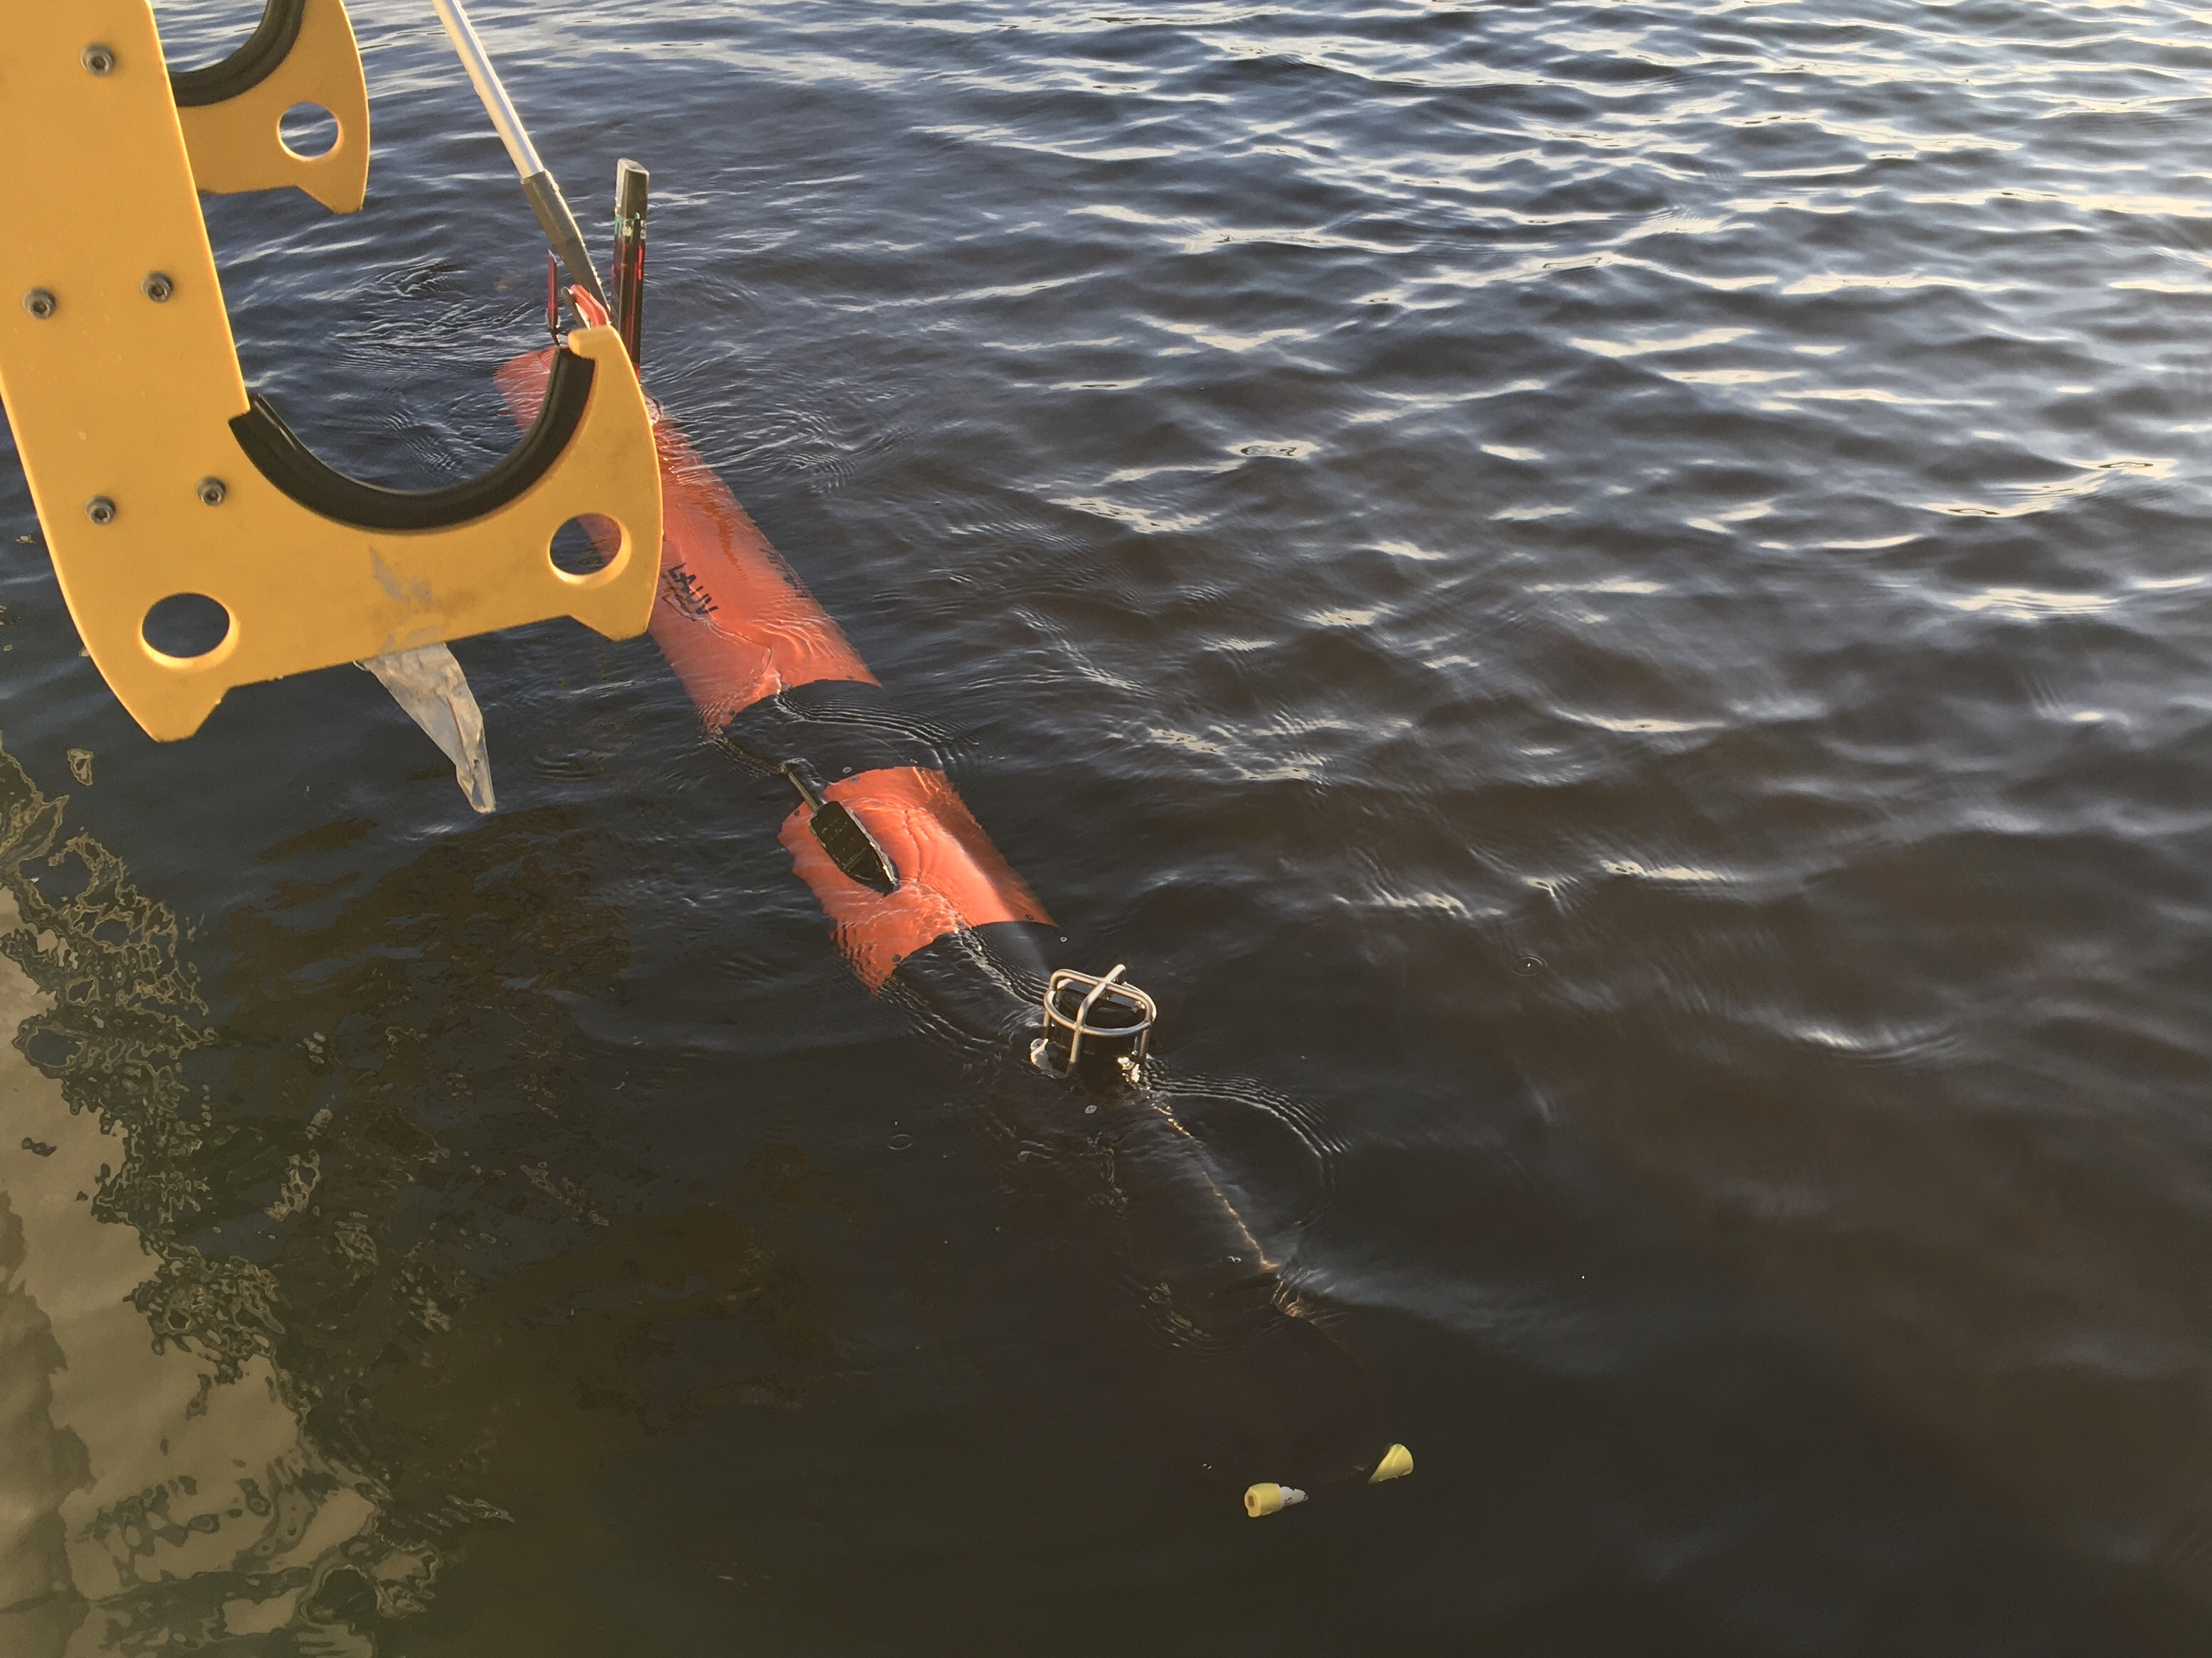
\includegraphics[width=\linewidth]{figures/Roald.jpeg}}
\caption{The Light Autonomous Underwater Vehicle (LAUV) Roald, used in the AILARON project, being picked up at the end of a mission in the Trondheim fjord.}
\label{fig:roald}
\end{figure}

\begin{figure}[tbp]
\centerline{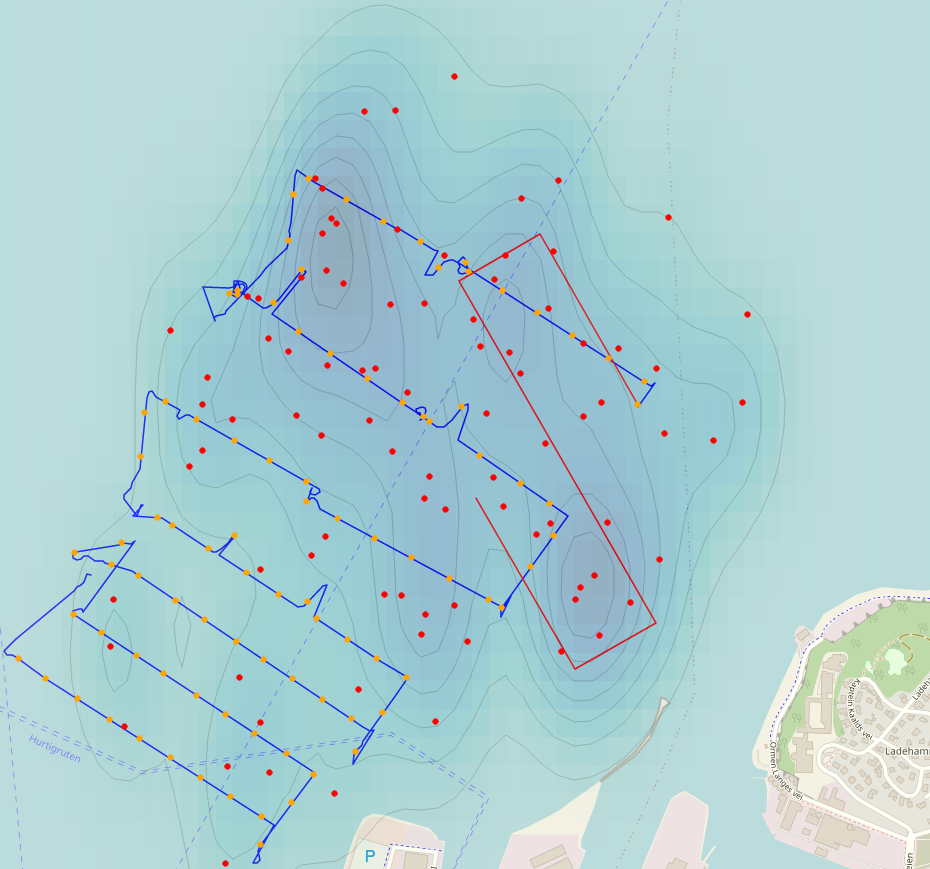
\includegraphics[width=\linewidth]{figures/munkholmen_planned_path.png}}
\caption{The AUV has traversed the blue path and gathered data (orange points), which has been transported with the current, and are now estimated to be located at the red points.
The contour shows the predicted concentration for which the red path is maximising expected measured concentration and minimising model variance.}
\label{fig:munkholmen}
\end{figure}

The next step is to perform new experiments with the AUV operating autonomously.
\section*{Acknowledgment}
This work was supported by the Research Council of Norway through the FRINATEK/IKTPLUSS program, project number 262701.
\end{document}
